\documentclass[10pt,
  aspectratio=169,
  serif,
  mathserif,
  professionalfont,
  compress,
  handout,
  % table,
  % svgnames
  ]{beamer}\usepackage[]{graphicx}\usepackage[]{color}
% maxwidth is the original width if it is less than linewidth
% otherwise use linewidth (to make sure the graphics do not exceed the margin)
\makeatletter
\def\maxwidth{ %
  \ifdim\Gin@nat@width>\linewidth
    \linewidth
  \else
    \Gin@nat@width
  \fi
}
\makeatother

\definecolor{fgcolor}{rgb}{1, 1, 0.941}
\newcommand{\hlnum}[1]{\textcolor[rgb]{0.804,0.718,0.71}{#1}}%
\newcommand{\hlstr}[1]{\textcolor[rgb]{0.604,0.753,0.804}{#1}}%
\newcommand{\hlcom}[1]{\textcolor[rgb]{0.439,0.502,0.565}{#1}}%
\newcommand{\hlopt}[1]{\textcolor[rgb]{1,1,0.941}{#1}}%
\newcommand{\hlstd}[1]{\textcolor[rgb]{1,1,0.941}{#1}}%
\newcommand{\hlkwa}[1]{\textcolor[rgb]{0.941,0.902,0.549}{#1}}%
\newcommand{\hlkwb}[1]{\textcolor[rgb]{1,0.871,0.678}{#1}}%
\newcommand{\hlkwc}[1]{\textcolor[rgb]{0.545,0.941,0.702}{#1}}%
\newcommand{\hlkwd}[1]{\textcolor[rgb]{0.545,0.941,0.902}{#1}}%
\let\hlipl\hlkwb

\usepackage{framed}
\makeatletter
\newenvironment{kframe}{%
 \def\at@end@of@kframe{}%
 \ifinner\ifhmode%
  \def\at@end@of@kframe{\end{minipage}}%
  \begin{minipage}{\columnwidth}%
 \fi\fi%
 \def\FrameCommand##1{\hskip\@totalleftmargin \hskip-\fboxsep
 \colorbox{shadecolor}{##1}\hskip-\fboxsep
     % There is no \\@totalrightmargin, so:
     \hskip-\linewidth \hskip-\@totalleftmargin \hskip\columnwidth}%
 \MakeFramed {\advance\hsize-\width
   \@totalleftmargin\z@ \linewidth\hsize
   \@setminipage}}%
 {\par\unskip\endMakeFramed%
 \at@end@of@kframe}
\makeatother

\definecolor{shadecolor}{rgb}{.97, .97, .97}
\definecolor{messagecolor}{rgb}{0, 0, 0}
\definecolor{warningcolor}{rgb}{1, 0, 1}
\definecolor{errorcolor}{rgb}{1, 0, 0}
\newenvironment{knitrout}{}{} % an empty environment to be redefined in TeX

\usepackage{alltt}

% Tamanho de fonte e distância entre linhas.
\renewenvironment{knitrout}{
  \renewcommand{\baselinestretch}{0.75}%\tiny
}{}

%-----------------------------------------------------------------------
% Pacotes padrões.

% Fontes.
\usepackage{palatino}
\usepackage{eulervm}
\usepackage{inconsolata}

% Esses pacotes dão clash.
% http://tex.stackexchange.com/questions/51488/option-clash-with-xcolor-and-tikz
% \usepackage{xcolor} %% opções no \documentclass{} para evitar clash.
% \definecolor{mycolor}{rgb}{0.13,0.53,0.53}
% \definecolor{mycolor2}{rgb}{0.725,0,0.18}

\usepackage{hyperref}
 \hypersetup{colorlinks, allcolors=., urlcolor=structure}
% \hypersetup{colorlinks}

\usepackage[brazil]{babel}
\usepackage[utf8]{inputenc}
\usepackage{graphicx}
\usepackage{amsmath, amsfonts, amssymb, amsxtra, amsthm, icomma}
\usepackage{geometry, calc, setspace, indentfirst}
% \usepackage{colortbl}
\usepackage{enumerate}
\usepackage{float}

\usepackage{subfigure}

\usepackage[hang]{caption}
\captionsetup{font=footnotesize,
  labelfont=footnotesize,
  labelsep=period}

% Listas em duas colulas.
\usepackage{multicol}
\newenvironment{itemize2}{%
  \vspace*{-1em}
  \begin{itemize}
    \begin{multicols}{2}
    }{%
    \end{multicols}
  \end{itemize}
}

% Texto no corpo do beamer justificado.
\usepackage{ragged2e}
\justifying

%-----------------------------------------------------------------------

% A lot of options:
% http://latex-community.org/forum/viewtopic.php?f=55&t=17646
\useoutertheme[
  width=60pt,
  height=30pt,
  right,
  hideothersubsections
  ]{sidebar}

\makeatletter
\setbeamertemplate{caption}[numbered]
\setbeamertemplate{section in toc}[sections numbered]
\setbeamertemplate{subsection in toc}[subsections numbered]
\setbeamertemplate{sections/subsections in toc}[ball]{}
\setbeamertemplate{section in sidebar right}[sections numbered]
%\setbeamertemplate{frametitle continuation}{\gdef\beamer@frametitle{}}
\setbeamertemplate{navigation symbols}{} %% Retira a barra de navegação.
% \setbeamertemplate{blocks}[rounded][shadow=FALSE]
% \setbeamercolor{block title}{fg=structure, bg=mycolor!20!white}
\makeatother

% Frames com sessão e/ou subsessão.
% \addtobeamertemplate{frametitle}{
%   \let\insertframetitle\insertsubsectionhead}{}
% \makeatletter
% \CheckCommand*\beamer@checkframetitle{
%   \@ifnextchar\bgroup\beamer@inlineframetitle{}}
% \renewcommand*\beamer@checkframetitle{
%   \global\let\beamer@frametitle\relax\@ifnextchar\bgroup
%   \beamer@inlineframetitle{}}
% \makeatother

\setbeamertemplate{frametitle}
{
    \nointerlineskip
    \begin{beamercolorbox}[sep=0.3cm,ht=1.8em,wd=\paperwidth]{frametitle}
        \vbox{}\vskip-2ex%
        \strut\insertframetitle\strut
        \vskip-0.8ex%
    \end{beamercolorbox}
}


%-----------------------------------------------------------------------
% Comandos.

\newcommand{\n}[1]{\textbf{#1}}

%-----------------------------------------------------------------------

\AtBeginSection[]{
  \begin{frame}[c,allowframebreaks]
    \begin{center}
      {\thesection} \\ \vspace{0.3cm}
      \parbox{0.6\textwidth}{
        \centering {\Large \textcolor{structure}{\insertsection}}}\\
    \end{center}
  \end{frame}
}

%-----------------------------------------------------------------------
% Definições dos proprietários.

\title[TH MCGLM]{
  \Large Testes de hipóteses em Modelos Multivariados de \\ Covariância Linear Generalizada}

\subtitle{ \\ Qualificação}

\author[Lineu Alberto]{\small
  Lineu Alberto Cavazani de Freitas \\
  Orientador: Prof. Dr. Wagner Hugo Bonat\\
  Co-orientador: Prof. Dr. Marco Antonio Zanata Alves
}

 \institute[UFPR]{
    PPG Informática %\\
%   Data Science \& Big Data \\
%   Universidade Federal do Paraná\\
% 
%   \vspace{1em}
%   \href{}{https://lineu96.github.io/st/}\\
%   \texttt{lineuacf@gmail.com}
 }
 \date{}

\logo{
\includegraphics[width=1.5cm]{img/dsbd1x4-rect.png}} 

\usebackgroundtemplate{
  
\includegraphics[width=\paperwidth]{img/ufpr-fundo.jpg}
}

\titlegraphic{
  \vspace{-1em}
  
\includegraphics[height=1.8cm]{img/capes_tp2.png}\hspace{2em}
  
\includegraphics[height=1.8cm]{img/ufpr-transparent.png}\hspace{2em}
  
\includegraphics[height=1.8cm]{img/dsbd-2x2-trans.png}
}

%---- preamble-refs.tex ------------------------------------------------

% Bibliography.

% %\usepackage[style=authoryear]{biblatex}
% \usepackage[authordate, bibencoding=auto, strict, backend=biber, natbib]{biblatex-chicago}
%
% % Use:
% %   \cite{<ref>}
% %   \parencite{<ref>}
% %   \fullcite{<ref>}
% %   \footfullcite{<ref>}
%
% % ATTENTION
% % Compilation: pdflatex > biber > pdflatex > pdflatex.
%
% % Calls refs.bib at preamble with:
% \addbibresource{config/refs.bib}

% abntex2cite -------------------------------

\usepackage[
  alf,
  abnt-emphasize=bf,
  abnt-etal-list=2,
  abnt-and-type=&]{abntex2cite}
% Use:
%   \cite{<ref>}
%   \citeonline{<ref>}

% ATTENTION
% Compilation: pdflatex > bibtex > pdflatex > pdflatex.

% Calls refs.bib at last frame with:
% \bibliography{config.refs}

\let\oldbibliography\thebibliography
\renewcommand{\thebibliography}[1]{%
  \oldbibliography{#1}%
  \setlength{\itemsep}{1em}%
}

%--------------------------------------------

%=======================================================================
%=======================================================================
\IfFileExists{upquote.sty}{\usepackage{upquote}}{}
\begin{document}

\frame{\titlepage}

% Tabela de conteúdo no início dos slides.
 \begin{frame}{Conteúdo}
   \small{\tableofcontents}
 \end{frame}

%-----------------------------------------------------------------------



%-----------------------------------------------------------------------

\section{Introdução}

%-----------------------------------------------------------------------

\begin{frame}
  \frametitle{Ciência de dados}
  \begin{itemize}
    \itemsep 2ex
  
  \item A ciência de dados é vista como um campo de estudo de natureza interdisciplinar que incorpora conhecimento de grandes áreas como estatística, ciência da computação e matemática \cite{ley2018makes}. 
  
  \item Tem diversos campos de interesse.

  \item Os métodos estatísticos são de fundamental importância em grande parte das etapas da ciência de dados \cite{weihs2018data}.
  
  \item Neste sentido, os modelos de regressão tem papel importante.
  
  \end{itemize}
\end{frame}

%-----------------------------------------------------------------------

\begin{frame}
  \frametitle{Modelos de regressão}

  Para entender minimamente um modelo de regressão, é necessário compreender o
  conceito de \textbf{fenômeno aleatório}, \textbf{variável aleatória} e \textbf{distribuição de probabilidade}.

  \begin{itemize}
    \itemsep 2ex

  \item Um \textbf{fenômeno aleatório} é situação na qual diferentes observações podem fornecer diferentes desfechos. 
  
  \item \textbf{Variáveis aleatórias} associam um valor numérico a cada desfecho possível do fenômeno. Podem ser discretas ou contínuas.
  
  \item Existem probabilidades associadas aos valores de uma variável aleatória. Estas probabilidades podem ser descritas por funções:
  
  \begin{itemize}
    \item Função de probabilidade, para variáveis aleatórias discretas.
    \item Função densidade de probabilidade, para variáveis aleatórias contínuas.
  \end{itemize}

  \end{itemize}
\end{frame}

%-----------------------------------------------------------------------

\begin{frame}
  
  \frametitle{Modelos de regressão}

  \begin{itemize}
    \itemsep 2ex

  \item Modelos probabilísticos que buscam descrever as probabilidades de variáveis aleatórias, as chamadas \textbf{distribuições de probabilidade}.
  
  \item Em problemas práticos, podemos buscar uma distribuição de probabilidades que melhor descreva o fenômeno de interesse. 
  
  \item Estas distribuições são descritas por funções. 
  
  \item Estas funções possuem parâmetros que controlam aspectos da distribuição.
  
  \item Os parâmetros são quantidades desconhecidas estimadas através dos dados.
  
  \end{itemize}

\end{frame}

%-----------------------------------------------------------------------

\begin{frame}
  \frametitle{Modelos de regressão}

  \begin{itemize}
    \itemsep 2ex

  \item Na análise de regressão busca-se modelar os parâmetros das distribuições de probabilidade como uma função de outras variáveis.
  
  \item Isto é feito através da decomposição do parâmetro da distribuição em outros parâmetros, chamados de parâmetros de regressão. 
  
  \item Assim, o objetivo dos modelos de regressão consiste em obter uma equação que explique a relação entre as variáveis explicativas e o parâmetro de interesse da distribuição de probabilidades selecionada para modelar a variável aleatória. 
  
  \item Em geral, o parâmetro de interesse da distribuição de probabilidades modelado em função das variávis explicativas é a média. 
  
  \end{itemize}
\end{frame}

%-----------------------------------------------------------------------

\begin{frame}
  \frametitle{Modelos de regressão}

  \begin{itemize}
    \itemsep 2ex

  \item O processo de análise via modelo de regressão parte de um conjunto de dados.
  
  \item Pode-se usar um modelo para modelar a relação entre a média de uma variável aleatória e um conjunto de variáveis explicativas. 
  
  \item Assume-se que a variável aleatória segue uma distribuição de probabilidades e que o parâmetro de média desta distribuição pode ser descrito por uma combinação linear de parâmetros de regressão associados às variáveis explicativas. 
  
  \item A obtenção destes parâmetros estimados se dá na chamada etapa de ajuste do modelo.
  
  \item Fazendo uso da equação resultante do processo é possível estudar a importância das variáveis explicativas sobre a resposta e realizar predições da variável resposta com base nos valores observados das variáveis explicativas. 
  
  \end{itemize}
\end{frame}

%-----------------------------------------------------------------------

\begin{frame}
  \frametitle{Modelos de regressão}

  \begin{itemize}
    \itemsep 2ex

  \item Existem modelos uni e multivariados. 
  
  \item Nos modelos univariados há apenas uma variável resposta e temos interesse em avaliar o efeito das variáveis explicativas sobre essa única resposta.
  
  \item No caso dos modelos multivariados há mais de uma resposta e o interesse passa a ser avaliar o efeito dessas variáveis sobre todas as respostas. 
  
  \item Existem inúmeras classes de modelos de regressão, mencionaremos neste trabalho três importantes classes: 
  \begin{itemize}
  \item Modelos lineares.
  \item Modelos lineares generalizados.
  \item Modelos multivariados de covariância linear generalizada. 
\end{itemize}

  \end{itemize}
\end{frame}


%-----------------------------------------------------------------------

\begin{frame}
  \frametitle{Modelo linear normal}

  \begin{itemize}
    \itemsep 2ex

  \item No cenário univariado, durante muitos anos o modelo linear normal \cite{galton} teve papel de destaque.
  
  \item Muito usado principalmente por suas facilidades computacionais. 
  
  \item Um dos pressupostos do modelo linear normal é de que a variável resposta, condicional às variáveis explicativas, segue a distribuição normal. 
  
  \item Quando tal pressuposto não era atendido, uma alternativa, por muito tempo adotada, foi buscar uma transformação da variável resposta, tal como a família de transformações Box-Cox \cite{boxcox64}. 
  
  \end{itemize}
\end{frame}

%-----------------------------------------------------------------------

\begin{frame}
  \frametitle{Modelos lineares generalizados}

  \begin{itemize}
    \itemsep 2ex

  \item O avanço computacional permitiu a proposição de modelos mais complexos, que necessitavam de processos iterativos para estimação dos parâmetros \cite{paula}. 
  
  \item A proposta de maior renome foram os modelos lineares generalizados (GLM) \cite{Nelder72}. 
  
  \item Essa classe de modelos permitiu a flexibilização da distribuição da variável resposta de tal modo que esta pertença à família exponencial de distribuições. 

  \item Em meio aos casos especiais de distribuições possíveis nesta classe de modelos estão a Bernoulli, binomial, Poisson, normal, gama, normal inversa, entre outras.  
  
  \end{itemize}
\end{frame}

%-----------------------------------------------------------------------

\begin{frame}
  \frametitle{Modelos multivariados de covariância linear generalizada}

  \begin{itemize}
    \itemsep 2ex

  \item Há casos em que são coletadas mais de uma resposta por unidade experimental e há o interesse de modelá-las em função de um conjunto de variáveis explicativas. 
  
  \item Neste cenário surgem os modelos multivariados de covariância linear generalizada (McGLM) \cite{Bonat16}. 
  
  \item Esta classe pode ser vista com uma extensão multivariada dos GLMs que permite lidar com múltiplas respostas de diferentes naturezas e, de alguma forma, correlacionadas. 

  \item O McGLM é uma classe flexível ao ponto de ser possível chegar a extensões multivariadas para modelos de medidas repetidas, séries temporais, dados longitudinais, espaciais e espaço-temporais.
  
  \end{itemize}
\end{frame}

%-----------------------------------------------------------------------

\begin{frame}
  \frametitle{Testes de hipóteses}

  \begin{itemize}
    \itemsep 2ex

  \item Em regressão, um interesse comum é o de verificar se a retirada de determinada variável explicativa do modelo geraria uma perda no ajuste. 
  
  \item Isto é feito através dos chamados testes de hipóteses. 

  \item Testes de hipóteses são ferramentas estatísticas que auxiliam no processo de tomada de decisão sobre valores desconhecidos (parâmetros) estimados por meio de uma amostra (estimativas).
  
  \item Podemos atribuir a teoria, formalização e filosofia dos testes de hipótese a Neyman, Pearson e Fisher.
  
  \end{itemize}
\end{frame}

%-----------------------------------------------------------------------

\begin{frame}
  \frametitle{Testes de hipóteses}

No contexto de modelos de regressão, três testes de hipóteses são comuns, todos baseados na função de verossimilhança: 

\begin{itemize}
  \item O teste da razão de verossimilhanças \cite{trv}.
  \item O teste Wald \cite{wald}.
  \item O teste do multiplicador de lagrange, também conhecido como teste escore \cite{score1}, \cite{score2}, \cite{score3}.
\end{itemize}


\end{frame}

%-----------------------------------------------------------------------

\begin{frame}
  \frametitle{Técnicas baseadas em testes de hipóteses}

  \begin{itemize}
    \itemsep 2ex

  \item Existem técnicas como a análise de variância (ANOVA) \cite{anova_fisher}. 
  
  \item O objetivo da técnica é a avaliação do efeito de cada uma das variáveis explicativas sobre a resposta. 

  \item Isto é feito através da comparação via testes de hipóteses entre modelos com e sem cada uma das variáveis explicativas.

  \item Permite que seja possível avaliar se a retirada de cada uma das variáveis gera um modelo significativamente pior quando comparado ao modelo com a variável. 

  \item Para o caso multivariado extende-se a técnica para a análise de variância multivariada \cite{manova}, a MANOVA. 

  \end{itemize}

\end{frame}

%-----------------------------------------------------------------------

\begin{frame}
  \frametitle{Proposta}

Objetivos gerais:

  \begin{itemize}
    \itemsep 2ex

  \item Considerando os McGLMs, não há discussão a respeito da construção de testes de hipóteses.
  
  \item Nosso objetivo geral é o desenvolvimento de testes de hipóteses para os McGLMs.

  \item Buscamos propor uma adaptação do teste de Wald clássico utilizado em modelos lineares para os McGLMs. 

  \end{itemize}

\end{frame}

%-----------------------------------------------------------------------

\begin{frame}
  \frametitle{Proposta}

Objetivos específicos: 

  \begin{itemize}
    \itemsep 2ex

  \item Adaptar o teste Wald para realização de testes de hipóteses gerais sobre parâmetros de McGLMs. 
  
  \item Implementar funções para efetuar tais testes, bem como funções para efetuar ANOVAs e MANOVAs para os McGLMs. 

  \item Avaliar as propriedades e comportamento dos testes propostos com base em estudos de simulação.

  \item Avaliar o potencial de aplicação das metodologias discutidas com base na aplicação a conjuntos de dados reais.

  \end{itemize}

\end{frame}

%-----------------------------------------------------------------------

\section{Revisão de literatura}

%-----------------------------------------------------------------------

\begin{frame}
  \frametitle{Revisão de literatura}
  
  A revisão de literatura compreende 3 temas:
  
  \begin{itemize}
    \itemsep 2ex
  \item Modelos multivariados de covariância linear generalizada. 
  \item Testes de hipóteses.
  \item ANOVA \& MANOVA.
  \end{itemize}
\end{frame}

%-----------------------------------------------------------------------

\subsection{McGLM}

%-----------------------------------------------------------------------

\begin{frame}[c, allowframebreaks]

\begin{center}

  {\normalsize \href{https://lineu96.github.io/st/}{Modelos Multivariados de Covariância Linear Generalizada}}
  
\end{center}

\end{frame}

%-----------------------------------------------------------------------

\begin{frame}
  \frametitle{Modelos multivariados de covariância linear generalizada}
  \begin{itemize}
    \itemsep 2ex
  
  \item Os GLMs são uma forma de modelagem para lidar com apenas uma resposta para dados de diferentes naturezas.  
  
  \item É uma classe de modelos flexível e aplicável a diversos tipos de problema.  
  
  \item Apresenta três importantes restrições:
    \begin{itemize}
      \item A incapacidade de lidar com observações dependentes. 
      \item A incapacidade de lidar com múltiplas respostas simultaneamente.
      \item Leque reduzido de distribuições disponíveis. 
    \end{itemize}

  \item Os McGLMs contornam estas restrições.
  
  \item Vamos discutir os McGLM como uma extensão dos GLM, seguindo as ideias de \cite{Bonat16} . 
  
  \end{itemize}
\end{frame}

%-----------------------------------------------------------------------

\begin{frame}
  \frametitle{GLM}
  
  Considere:

\begin{itemize}
  \item $\boldsymbol{Y}$ um vetor $N \times 1$ de valores observados da variável resposta.
  
  \item $\boldsymbol{X}$ uma matriz de delineamento $N \times k$
  
  \item $\boldsymbol{\beta}$ um vetor de parâmetros de regressão $k \times 1$. 
\end{itemize}

\end{frame}

%-----------------------------------------------------------------------

\begin{frame}
  \frametitle{GLM}

um GLM pode ser descrito da forma

\begin{equation}
      \begin{aligned}
        \mathrm{E}(\boldsymbol{Y}) &=
         \boldsymbol{\mu} =
            g^{-1}(\boldsymbol{X} \boldsymbol{\beta}),
            \\
        \mathrm{Var}(\boldsymbol{Y}) &=
          \Sigma =
          \mathrm{V}\left(\boldsymbol{\mu}; p\right)^{1/2}\left(\tau_0\boldsymbol{I}\right)\mathrm{V}\left(\boldsymbol{\mu}; p\right)^{1/2},
      \end{aligned}
\end{equation}

Em que:

  \begin{itemize}
    \itemsep 2ex
  
  \item $g(.)$ é a função de ligação. 
  
  \item $\mathrm{V}\left(\boldsymbol{\mu}; p\right)$ é uma matriz diagonal em que as entradas principais são dadas pela função de variância aplicada ao vetor $\boldsymbol{\mu}$. 
  
  \item $p$ é o parâmetro de potência. 
  
  \item $\tau_0$ o parâmetro de dispersão. 
  
  \item $\boldsymbol{I}$ é a matriz identidade de ordem $N\times N$.
  
  \end{itemize}
\end{frame}

%-----------------------------------------------------------------------

\begin{frame}

  \frametitle{GLM}
  
  \begin{enumerate}
  \item Função de variância potência \cite{Jorgensen87} e \cite{Jorgensen97}. 
  
    \begin{itemize}
      \item Família Tweedie de distribuições.
      \item $\vartheta\left(\boldsymbol{\mu}; p\right) = \mu^p$
      \item Casos particulares: normal ($p$ = 0), Poisson ($p$ = 1), gama ($p$ = 2) e normal inversa ($p$ = 3).
    \end{itemize}

  
  \item Função de dispersão Poisson–Tweedie \cite{Jorgensen15}.
  
    \begin{itemize}
      \item Família Poisson-Tweedie de distribuições.
      \item $\vartheta\left(\boldsymbol{\mu}; p\right) = \mu + \mu^p$
      \item Casos particulares: Hermite ($p$ = 0), Neyman tipo A ($p$ = 1), binomial negativa ($p$ = 2) e Poisson–inversa gaussiana (p = $3$)
      
    \end{itemize}

  \item Função de variância binomial. 
  
    \begin{itemize}
      \item $\vartheta(\boldsymbol{\mu}) = \mu(1 - \mu)$
      \item Acomoda respostas binárias ou restritas a um intervalo.
    \end{itemize}

\end{enumerate}

\end{frame}

%-----------------------------------------------------------------------

\begin{frame}
  \frametitle{cGLM}
  \begin{itemize}
    \itemsep 2ex
  
  \item Alternativa para problemas em que a suposição de independência entre as observações não é atendida. 
  
  \item A solução proposta é substituir a matriz identidade $\boldsymbol{I}$ da equação que descreve a matriz de variância e covariância por uma matriz não diagonal $\boldsymbol{\Omega({\tau})}$. 
  
  \item A matriz $\boldsymbol{\Omega({\tau})}$ é descrita como uma combinação de matrizes conhecidas \cite{Anderson73} \cite{Pourahmadi00}.
  
  \end{itemize}
\end{frame}

%-----------------------------------------------------------------------

\begin{frame}
  \frametitle{cGLM}
  
  A matriz $\boldsymbol{\Omega({\tau})}$ pode ser escrita como:

\begin{equation}
h\left \{ \boldsymbol{\Omega}(\boldsymbol{\tau}) \right \} = \tau_0Z_0 + \ldots + \tau_DZ_D,
\end{equation}

em que 
  
  \begin{itemize}
    \itemsep 2ex
    
  \item $h(.)$ é a função de ligação de covariância. 
  
  \item $Z_d$ com $d$ = 0,$\ldots$, D são matrizes que representam a estrutura de covariância presente nos dados. 
  
  \item $\boldsymbol{\tau}$ = $(\tau_0, \ldots, \tau_D)$ é um vetor $(D + 1) \times 1$ de parâmetros de dispersão. 
  
  \item Tal estrutura pode ser vista como um análogo ao preditor linear para a média e foi nomeado como preditor linear matricial. 
  
  \end{itemize}

\end{frame}

%-----------------------------------------------------------------------

\begin{frame}
  \frametitle{McGLM}
  \begin{itemize}
    \itemsep 2ex
  
  \item Pode ser entendido como uma extensão multivariada do cGLM. 
  
  \item Contorna as principais restrições presentes nos GLM. 

  \end{itemize}
  
  Considere
  
  \begin{itemize}
  \item $\boldsymbol{Y}_{N \times R} = \left \{ \boldsymbol{Y}_1, \dots, \boldsymbol{Y}_R \right \}$ uma matriz de variáveis resposta
  
  \item $\boldsymbol{M}_{N \times R} = \left \{ \boldsymbol{\mu}_1, \dots, \boldsymbol{\mu}_R \right \}$ uma matriz de valores esperados.
  
  \item $\Sigma_b$, uma martiz de ordem $R \times R$, que descreve a correlação entre as variáveis resposta.
  
  \item Cada uma das variáveis resposta tem sua própria matriz de variância e covariância:

\begin{equation}
\Sigma_r =
\mathrm{V}_r\left(\boldsymbol{\mu}_r; p\right)^{1/2}\boldsymbol{\Omega}_r\left(\boldsymbol{\tau}\right)\mathrm{V}_r\left(\boldsymbol{\mu}_r; p\right)^{1/2}.
\end{equation}
 
\end{itemize}

\end{frame}

%-----------------------------------------------------------------------

\begin{frame}
  \frametitle{McGLM}
  
  Um MCGLM é descrito como

\begin{equation}
\label{eq:mcglm}
      \begin{aligned}
        \mathrm{E}(\boldsymbol{Y}) &=
          \boldsymbol{M} =
            \{g_1^{-1}(\boldsymbol{X}_1 \boldsymbol{\beta}_1),
            \ldots,
            g_R^{-1}(\boldsymbol{X}_R \boldsymbol{\beta}_R)\}
          \\
        \mathrm{Var}(\boldsymbol{Y}) &=
          \boldsymbol{C} =
            \boldsymbol{\Sigma}_R \overset{G} \otimes
            \boldsymbol{\Sigma}_b,
      \end{aligned}
\end{equation}

em que 
  
  \begin{itemize}
    
    \itemsep 0.5ex
    
  \item $\boldsymbol{\Sigma}_R \overset{G} \otimes \boldsymbol{\Sigma}_b = \mathrm{Bdiag}(\tilde{\boldsymbol{\Sigma}}_1, \ldots, \tilde{\boldsymbol{\Sigma}}_R) (\boldsymbol{\Sigma}_b \otimes \boldsymbol{I}) \mathrm{Bdiag}(\tilde{\boldsymbol{\Sigma}}_1^\top, \ldots, \tilde{\boldsymbol{\Sigma}}_R^\top)$ é o produto generalizado de Kronecker. 
  
  \item A matriz $\tilde{\boldsymbol{\Sigma}}_r$ denota a matriz triangular inferior da decomposição de Cholesky da matriz ${\boldsymbol{\Sigma}}_r$. 
  
  \item O operador $\mathrm{Bdiag}$ denota a matriz bloco-diagonal. 
  
  \item $\boldsymbol{I}$ uma matriz identidade $N \times N$.
  
  \item A metodologia do McGLM está implementada no pacote \emph{mcglm} \cite{mcglm} do software R.

  \end{itemize}
  
\end{frame}

%-----------------------------------------------------------------------

\begin{frame}[c, allowframebreaks]

\begin{center}

  {\normalsize \href{https://lineu96.github.io/st/}{Estimação e inferência}}
  
\end{center}

\end{frame}

%-----------------------------------------------------------------------

\begin{frame}

\frametitle{Funções de estimação}

As funções de estimação para os parâmetros de regressão (função quasi-score) e de dispersão (função de estimação de Pearson) são dadas por:

\begin{center}
$\psi_{\boldsymbol{\beta}}(\boldsymbol{\beta}, \boldsymbol{\lambda}) = \boldsymbol{D}^\top \boldsymbol{C}^{-1}(\mathcal{Y} - \mathcal{M})$

$\psi_{\boldsymbol{\lambda}_i}(\boldsymbol{\beta}, \boldsymbol{\lambda}) = \mathrm{tr}(W_{\boldsymbol{\lambda}i} (\boldsymbol{r}^\top\boldsymbol{r} - \boldsymbol{C})),  i = 1,.., Q$
\end{center}

Em que:

\begin{itemize}
  
  \item \normalsize $\boldsymbol{\beta}_r$ denota um vetor $k_r \times 1$ de parâmetros de regressão.
  
  \item \normalsize $\boldsymbol{\lambda}$ é um vetor $Q \times 1$ de parâmetros de dispersão.
  
  \item \normalsize $\mathcal{Y}$ é um vetor $NR \times 1$ com os valores da matriz de variáveis respostas $Y_{N \times R}$ empilhados.
  
  \item \normalsize $\mathcal{M}$ é um vetor $NR \times 1$ com os valores da matriz de valores esperados $M_{N \times R}$ empilhados.
  
  \item \normalsize $\boldsymbol{D} = \nabla_{\boldsymbol{\beta}} \mathcal{M}$ 
é uma matriz $NR \times K$, e $\nabla_{\boldsymbol{\beta}}$ denota o 
operador gradiente.
  
  \item \normalsize $W_{\boldsymbol{\lambda}i} = -\frac{\partial
    \boldsymbol{C}^{-1}}{\partial \boldsymbol{\lambda}_i}$ 
    
  \item \normalsize $\boldsymbol{r} = (\mathcal{Y} - \mathcal{M})$
  
\end{itemize}

\end{frame}

% -----------------------------------------------------------------

\begin{frame}

\frametitle{Distribuição assintótica e algoritmo de estimação}

\begin{itemize}

  \item Para resolver o sistema de equações $\psi_{\boldsymbol{\beta}} = 0$ e $\psi_{\boldsymbol{\lambda}} = 0$ faz-se uso do algoritmo Chaser modificado:

$$
\begin{matrix}
\boldsymbol{\beta}^{(i+1)} = \boldsymbol{\beta}^{(i)}- S_{\boldsymbol{\beta}}^{-1} \psi \boldsymbol{\beta} (\boldsymbol{\beta}^{(i)}, \boldsymbol{\lambda}^{(i)}), \\ 
\boldsymbol{\lambda}^{(i+1)} = \boldsymbol{\lambda}^{(i)}\alpha S_{\boldsymbol{\lambda}}^{-1} \psi \boldsymbol{\lambda} (\boldsymbol{\beta}^{(i+1)}, \boldsymbol{\lambda}^{(i)}).
\end{matrix}
$$

  \item Seja $\boldsymbol{\hat{\theta}} = (\boldsymbol{\hat{\beta}^{\top}}, \boldsymbol{\hat{\lambda}^{\top}})^{\top}$ o estimador baseado em funções de estimação de $\boldsymbol{\theta}$.
  
  \item A distribuição assintótica de $\boldsymbol{\hat{\theta}}$ é:

$$
\boldsymbol{\hat{\theta}} \sim N(\boldsymbol{\theta}, J_{\boldsymbol{\theta}}^{-1}),
$$

\noindent $J_{\boldsymbol{\theta}}^{-1}$ é a inversa da matriz de informação de Godambe, dada por
  
$$J_{\boldsymbol{\theta}}^{-1} = S_{\boldsymbol{\theta}}^{-1} V_{\boldsymbol{\theta}} S_{\boldsymbol{\theta}}^{-\top},$$ 

\noindent em que $S_{\boldsymbol{\theta}}^{-\top} = (S_{\boldsymbol{\theta}}^{-1})^{\top}.$

\end{itemize}

\end{frame}

%-----------------------------------------------------------------------

\subsection{Testes de hipóteses}

%-----------------------------------------------------------------------

\begin{frame}[c, allowframebreaks]

\begin{center}

  {\normalsize \href{https://lineu96.github.io/st/}{Testes de hipóteses}}
  
\end{center}

\end{frame}

%-----------------------------------------------------------------------

\begin{frame}
  \frametitle{Testes de hipóteses}
  \begin{itemize}
    \itemsep 2ex
  
  \item Um dos objetivos principais da análise estatística é inferir conclusões válidas a respeito de uma população por meio do estudo de uma amostra. 
  
  \item Problemas de inferência estatística são:
    \begin{enumerate}
      
      \item Estimação de parâmetros com base em informação amostral.
      
      \item Testes de hipóteses:
        \begin{itemize}
          \item Com base na evidência amostral, podemos considerar que dado parâmetro tem determinado valor?
        \end{itemize}
    
    \end{enumerate}

  
  \item Uma hipótese estatística é uma afirmação ou conjetura sobre parâmetros.
  
  \end{itemize}
  
\end{frame}

%-----------------------------------------------------------------------

\begin{frame}
  \frametitle{Testes de hipóteses}
  \begin{itemize}
    \itemsep 2ex
  
  \item São postuladas 2 hipóteses, chamadas de nula e alternativa.
  
  \item Avalia-se uma estatística de teste. 
  
  \item Com base no valor da estatística e de acordo com sua distribuição de probabilidade, toma-se a decisão de rejeitar ou não rejeitar a hipótese nula.
    
  \item Seja $\theta$ um parâmetro, um teste de hipóteses sobre $\theta$ é dado por:
  
  $$
\left\{\begin{matrix}
H_0: \theta = \theta_0 \\ 
H_1: \theta \neq \theta_0
\end{matrix}\right.
$$  
  
  \end{itemize}


\end{frame}

%-----------------------------------------------------------------------

\begin{frame}
  \frametitle{Testes de hipóteses}
  
  Desfechos possíveis:
  
  \begin{table}[]
\begin{tabular}{l|cc}
\hline
\multicolumn{1}{c|}{}    & \textbf{Rejeita $H_0$} & \textbf{Não Rejeita $H_0$} \\ \hline
\textbf{$H_0$ verdadeira} & Erro tipo I           & Decisão correta           \\
\textbf{$H_0$ falsa}      & Decisão correta       & Erro tipo II              \\ \hline
\end{tabular}
\caption{Desfechos possíveis em um teste de hipóteses}
\label{tab:my-table}
\end{table}
  
  \begin{itemize}
    \itemsep 2ex
  
  \item A probabilidade do erro do tipo I recebe o nome de nível de significância.
  
  \item A probabilidade de se rejeitar a hipótese nula quando a hipótese alternativa é verdadeira (rejeitar corretamente $H_0$) recebe o nome de poder do teste.
  
  \item A probabilidade de a estatística de teste tomar um valor igual ou mais extremo do que aquele que foi observado recebe o nome de p-valor.
    
  \end{itemize}

\end{frame}

%-----------------------------------------------------------------------

\begin{frame}
  \frametitle{Testes de hipóteses}
  \begin{itemize}
    \itemsep 2ex
  
  \item Em modelos de regressão, testes de hipóteses são usados para verificar se a retirada de determinada variável explicativa do modelo geraria uma perda no ajuste.
  
  \item Os três testes mais usados para este fim são:

    \begin{itemize}
      \item O teste da razão de verossimilhanças \cite{trv}.
      \item O teste Wald \cite{wald}.
      \item O teste do multiplicador de lagrange, também conhecido como teste escore \cite{score1}, \cite{score2}, \cite{score3}.
    \end{itemize}
  
  \item Todos eles são baseados na função de verossimilhança dos modelos.
  
  
  \item São assintóticamente equivalentes. Em amostras finitas estes testes podem apresentar resultados diferentes \cite{conflict}.
  
  \end{itemize}
  
\end{frame}

%-----------------------------------------------------------------------

\begin{frame}
  \frametitle{Teste da razão de verossimilhanças}

  \begin{itemize}
    \itemsep 2ex

  \item O teste da razão de verossimilhanças é efetuado a partir de dois modelos com o objetivo de compará-los. 
  
  \item A ideia consiste em obter um modelo com todas as variáveis explicativas e um segundo modelo sem algumas dessas variáveis. 

  \item O teste é usado para comparar estes modelos através da diferença do logaritmo da função de verossimilhança. 

  \item Caso essa diferença seja estatísticamente significativa, significa que a retirada das variáveis do modelo completo prejudicam o ajuste. 

  \item Caso não seja observada diferença entre o modelo completo e o restrito, significa que as variáveis retiradas não geram perda na qualidade e, por este motivo, tais variáveis podem ser descartadas.

  \end{itemize}


\end{frame}

%-----------------------------------------------------------------------

\begin{frame}
  \frametitle{Teste da razão de verossimilhanças}

\begin{itemize}
  \itemsep 2ex

  \item Considere 2 modelos de regressão encaixados em que a diferença entre o número de parâmetros entre os modelos é igual a $q$.
  
  \item Considere $\boldsymbol{\beta}$ um vetor de parâmetros de regressão e $\boldsymbol{0}$ o vetor nulo.
  
  \item As hipóteses podem ser descritas como

$$
\left\{\begin{matrix}
H_0: \boldsymbol{\beta} = \boldsymbol{0} \\ 
H_1: \boldsymbol{\beta} \neq \boldsymbol{0}
\end{matrix}\right.
$$

  \item A estatística de teste é dada por:
  $$
LRT = -2log\left ( L_0/L_1 \right ),
$$

em que $L_0$ representa a verossimilhança do modelo restrito e $L_1$ a verossimilhança do irrestrito.

 \item  LRT \sim \chi^2_q.

\end{itemize}

\end{frame}

%-----------------------------------------------------------------------

\begin{frame}
  \frametitle{Teste Wald}

  \begin{itemize}
    \itemsep 2ex

  \item O teste Wald, requer apenas um modelo ajustado. 
  
  \item A ideia consiste em verificar se existe evidência para afirmar que um ou mais parâmetros são iguais a valores postulados. 

  \item O teste avalia quão longe o valor estimado está do valor postulado. 

  \item Utilizando o teste Wald é possível formular hipóteses para múltiplos parâmetros. 

  \end{itemize}

\end{frame}

%-----------------------------------------------------------------------

\begin{frame}
  \frametitle{Teste Wald}

\begin{itemize}
  \itemsep 2ex

  \item Considere um modelo de regressão ajustado com $p$ parâmetros.
  
  \item Considere $\boldsymbol{\beta}$ um vetor de parâmetros de regressão, em que as estimativas são dadas por $\boldsymbol{\hat\beta}$ e $\boldsymbol{c}$ um vetor de valores postulados de dimensão $q$.
  
  \item Considere $\boldsymbol{L}$uma matriz de especificação das hipóteses, de dimensão $qxp$.
  
  \item As hipóteses podem ser descritas como

$$
\left\{\begin{matrix}
H_0: \boldsymbol{L}\boldsymbol{\beta} = \boldsymbol{c} \\ 
H_1: \boldsymbol{L}\boldsymbol{\beta} \neq \boldsymbol{c}
\end{matrix}\right.
$$

  \item A estatística de teste é dada por:
  $$
WT = (\boldsymbol{L\hat\beta} - \boldsymbol{c})^T \ (\boldsymbol{L \ Var^{-1}(\hat\beta) \ L^T})^{-1} \ (\boldsymbol{L\hat\beta} - \boldsymbol{c}).
$$

 \item  WT \sim \chi^2_q.

\end{itemize}

\end{frame}

%-----------------------------------------------------------------------

\begin{frame}
  \frametitle{Teste Escore}

  \begin{itemize}
    \itemsep 2ex

  \item O teste do multiplicador de lagrange ou teste score, tal como o teste Wald, requer apenas um modelo ajustado. 
  
  \item No caso do teste escore o modelo ajustado não possui o parâmetro de interesse e o que é feito é testar se adicionar esta variável omitida resultará em uma melhora significativa no modelo. 

  \item Isto é feito com base na inclinação da função de verossimilhança, esta inclinação é usada para estimar a melhoria no modelo caso as variáveis omitidas fossem incluídas. 

  \end{itemize}

\end{frame}

%-----------------------------------------------------------------------

\begin{frame}
  \frametitle{Teste Escore}

\begin{itemize}
  \itemsep 2ex

  \item Considere um modelo de regressão ajustado com $p$ parâmetros.
  
  \item Considere $\boldsymbol{\beta}$ um vetor de parâmetros de regressão, em que as estimativas são dadas por $\boldsymbol{\hat\beta}$ e $\boldsymbol{0}$ o vetor nulo.
  
  \item As hipóteses podem ser descritas como

$$
\left\{\begin{matrix}
H_0: \boldsymbol{\beta} = \boldsymbol{0} \\ 
H_1: \boldsymbol{\beta} \neq \boldsymbol{0}
\end{matrix}\right.
$$

  \item A estatística de teste é dada por:

$$ LMT = \boldsymbol{S^{'}(\hat\beta}) \ \boldsymbol{Var(\hat\beta)} \ \boldsymbol{S(\hat\beta}).$$

Em que $S(\hat\beta)$ representa a função escore e $\boldsymbol{Var(\hat\beta)}$ a matriz de variâncias avaliadas sob o modelo restrito ($H_0$).

 \item  WT $\sim \chi^2_q$, em que $q$ representa o número de parâmetros fixados sob $H_0$.

\end{itemize}

\end{frame}

%-----------------------------------------------------------------------

\begin{frame}
  \frametitle{LRT, WT \& LMT}

\begin{figure} % Inicia o ambiente de figuras
  %\subfigure{ % Começa a incluir a figura fig1.pdf
  %  
\includegraphics[width=2cm]{img/logo.png}
  %} % Termina de incluir a figura fig1.pdf
  \subfigure{ % Começa a incluir a figura fig2.pdf na mesma linha da figura fig1.pdf
    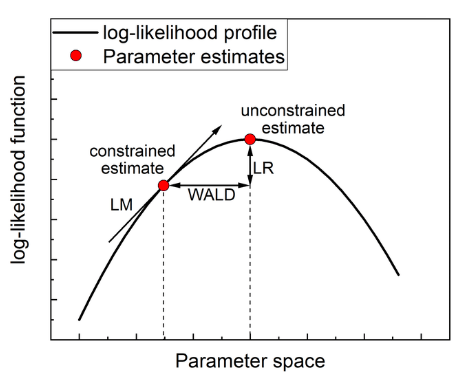
\includegraphics[width=8cm]{img/tests.png}
  } % Termina de incluir a figura fig2.pdf
  %\subfigure{ % Começa a incluir a figura fig3.pdf na linha abaixo
  %  
\includegraphics[width=1.4cm]{img/dsbd-2x2-trans.png}
  %} % Termina de incluir a figura fig3.pdf
\end{figure} % Fecha o ambiente de figuras

\end{frame}

%-----------------------------------------------------------------------

\subsection{ANOVA \& MANOVA}

%-----------------------------------------------------------------------

\begin{frame}[c, allowframebreaks]

\begin{center}

  {\normalsize \href{https://lineu96.github.io/st/}{ANOVA \& MANOVA}}
  
\end{center}

\end{frame}

%-----------------------------------------------------------------------

\begin{frame}
  \frametitle{ANOVA \& MANOVA}

  \begin{itemize}
    \itemsep 2ex

  \item Formas de avaliar a significância de cada uma das variáveis de uma forma procedural.  
  
  \item Consiste em efetuar testes sucessivos impondo restrições ao modelo original. 

  \item O objetivo é testar se a ausência de determinada variável gera perda ao modelo. 
  
  \item Os resultados são sumarizados numa tabela, o chamado quadro de análise de variância, que contêm em cada linha: 
  
  \begin{enumerate}
  \item A variável.
  \item O valor de uma estatística de teste referente à hipótese de nulidade de todos os parâmetros associados à esta variável.
  \item Os graus de liberdade.
  \item O p-valor associado à hipótese testada naquela linha do quadro.
  \end{enumerate}


  \end{itemize}

\end{frame}

%-----------------------------------------------------------------------

\begin{frame}
  \frametitle{ANOVA \& MANOVA}

  \begin{itemize}
    \itemsep 2ex

  \item Na ANOVA \cite{anova_fisher}, avalia-se a relevância das variáveis sobre uma única resposta. 

  \item Na MANOVA \cite{manova}, avalia-se a relevância das variáveis sobre mais de uma resposta. 

  \item Formas conhecidas de se elaborar o quadro são as chamadas ANOVAs do tipo I, II e III. 

  \item Esta nomenclatura vem do software estatístico SAS \cite{sas}. 

  \item No software R \cite{softwareR} as implementações dos diferentes tipos de análise de variância podem ser obtidas e usadas no pacote \emph{car} \cite{car}.
  
  \end{itemize}

\end{frame}

%-----------------------------------------------------------------------

\section{Proposta}

%-----------------------------------------------------------------------

\subsection{Adaptação do teste Wald para os McGLM}

%-----------------------------------------------------------------------

\begin{frame}[c, allowframebreaks]

\begin{center}

  {\normalsize \href{https://lineu96.github.io/st/}{Adaptação do teste Wald para os McGLMs}}
  
\end{center}

\end{frame}

% -----------------------------------------------------------------

\begin{frame}
\frametitle{Hipóteses}

As hipóteses a serem testadas podem ser escritas como:

$$H_0: \boldsymbol{L}\boldsymbol{\theta_{\beta,\tau,p}} = \boldsymbol{c} \ vs \ H_1: \boldsymbol{L}\boldsymbol{\theta_{\beta,\tau,p}} \neq \boldsymbol{c}.$$ 

Em que: 

\begin{itemize}
  
  \item Em que $\boldsymbol{L}$ é a matriz de especificação das hipóteses a serem testadas, tem dimensão $s \times h$. 
  
  \item $\boldsymbol{\theta_{\beta,\tau,p}}$ é o vetor de dimensão $h \times 1$ de parâmetros de regressão, dispersão e potência do modelo. 
  
  \item $\boldsymbol{c}$ é um vetor de dimensão $s \times 1$ com os valores sob hipótese nula.

\end{itemize}

\end{frame}

% -----------------------------------------------------------------

\begin{frame}
\frametitle{Estatística de teste}

A generalização da estatística de teste para verificar a validade de uma hipótese sobre parâmetros de um McGLM é dada por:

$$W = (\boldsymbol{L\hat\theta_{\beta,\tau,p}} - \boldsymbol{c})^T \ (\boldsymbol{L \ J_{\boldsymbol{{\beta,\tau,p}}}^{-1} \ L^T})^{-1} \ (\boldsymbol{L\hat\theta_{\beta,\tau,p}} - \boldsymbol{c}).$$

Em que: 

\begin{itemize}
  \item $\boldsymbol{L}$ é a mesma matriz da especificação das hipóteses a serem testadas, tem dimensão $s \times h$. 

  \item $\boldsymbol{\hat\theta_{\beta,\tau,p}}$ é o vetor de dimensão $h \times 1$ com todas as estimativas dos parâmetros de regressão, dispersão e potência do modelo. 

  \item $\boldsymbol{c}$ é um vetor de dimensão $s \times 1$ com os valores sob hipótese nula. 

  \item E $J_{\boldsymbol{{\beta,\tau,p}}}^{-1}$ é a inversa da matriz de informação de Godambe desconsiderando os parâmetros de correlação, de dimensão $h \times h$. 

\end{itemize}

\end{frame}

% -----------------------------------------------------------------

\subsection{Exemplos de hipóteses}

% -----------------------------------------------------------------

\begin{frame}[c, allowframebreaks]

\begin{center}

  {\normalsize \href{https://lineu96.github.io/st/}{Exemplos de hipóteses nos McGLMs}}
  
\end{center}

\end{frame}

% -----------------------------------------------------------------

\begin{frame}

\frametitle{Exemplos de hipóteses}

Considere um modelo bivariado genérico, com preditor dado por:

$$g_r(\mu_r) = \beta_{r0} + \beta_{r1} x_1$$

\begin{itemize}
  
  \item O índice $r$ denota a variável resposta, r = 1,2.
  
  \item $\beta_{r0}$ representa o intercepto.
  
  \item $\beta_{r1}$ um parâmetro de regressão associado a uma variável $x_1$.
  
  \item Considere que cada resposta possui apenas um parâmetro de dispersão: $\tau_{r1}$.
  
  \item Considere que os parâmetros de potência foram fixados.
  
\end{itemize}

\end{frame}

% -----------------------------------------------------------------

\begin{frame}

\frametitle{Exemplo 1: único parâmetro}

Considere a hipótese:

$$H_0: \beta_{11} = 0 \ vs \ H_1: \beta_{11} \neq 0.$$

Esta hipótese pode ser reescrita na seguinte notação:

$$H_0: \boldsymbol{L}\boldsymbol{\theta_{\beta,\tau,p}} = \boldsymbol{c} \ vs \ H_1: \boldsymbol{L}\boldsymbol{\theta_{\beta,\tau,p}} \neq \boldsymbol{c}.$$ 

Em que:

\begin{itemize}
  
  \item $\boldsymbol{\theta_{\beta,\tau,p}^T}$ = $\begin{bmatrix} \beta_{10} \  \beta_{11} \ \beta_{20} \ \beta_{21} \ \tau_{11} \ \tau_{21} \end{bmatrix}$.


\item $\boldsymbol{L} = \begin{bmatrix} 0 & 1 & 0 & 0 & 0 & 0  \end{bmatrix}.$
 
\item $\boldsymbol{c}$ = $\begin{bmatrix} 0 \end{bmatrix}$, é o valor da hipótese nula. 

\end{itemize}

\end{frame}

% -----------------------------------------------------------------

\begin{frame}

\frametitle{Exemplo 2: múltiplos parâmetros}

Considere a hipótese:

$$H_0: \beta_{r1} = 0 \ vs \ H_1: \beta_{r1} \neq 0.$$ 

Ou, da mesma forma:

$$H_0: 
\begin{pmatrix}
\beta_{11} \\ 
\beta_{21}
\end{pmatrix} 
= 
\begin{pmatrix}
0 \\ 
0
\end{pmatrix}
\ vs \ 
H_1: 
\begin{pmatrix}
\beta_{11} \\ 
\beta_{21}
\end{pmatrix} 
\neq
\begin{pmatrix}
0 \\ 
0 
\end{pmatrix}.$$

\end{frame}

% -----------------------------------------------------------------

\begin{frame}

\frametitle{Exemplo 2: múltiplos parâmetros}

A hipótese pode ser reescrita na seguinte notação:

$$H_0: \boldsymbol{L}\boldsymbol{\theta_{\beta,\tau,p}} = \boldsymbol{c} \ vs \ H_1: \boldsymbol{L}\boldsymbol{\theta_{\beta,\tau,p}} \neq \boldsymbol{c}.$$ 

Em que:

\begin{itemize}
  
  \item $\boldsymbol{\theta_{\beta,\tau,p}^T}$ = $\begin{bmatrix} \beta_{10} \  \beta_{11} \ \beta_{20} \ \beta_{21} \ \tau_{11} \ \tau_{21} \end{bmatrix}$.


\item $\boldsymbol{L} = \begin{bmatrix} 0 & 1 & 0 & 0 & 0 & 0 \\
0 & 0 & 0 & 1 & 0 & 0 \end{bmatrix}$
 
\item $\boldsymbol{c} = \begin{bmatrix} 0 \\ 0 \end{bmatrix}$, é o valor da hipótese nula. 

\end{itemize}

\end{frame}

% -----------------------------------------------------------------

\begin{frame}

\frametitle{Exemplo 3: igualdade de efeitos}

Considere a hipótese:

$$H_0: \beta_{11} - \beta_{21} = 0 \ vs \ H_1: \beta_{11} - \beta_{21} \neq 0.$$

Esta hipótese pode ser reescrita na seguinte notação:

$$H_0: \boldsymbol{L}\boldsymbol{\theta_{\beta,\tau,p}} = \boldsymbol{c} \ vs \ H_1: \boldsymbol{L}\boldsymbol{\theta_{\beta,\tau,p}} \neq \boldsymbol{c}.$$ 

Em que:

\begin{itemize}
  
  \item $\boldsymbol{\theta_{\beta,\tau,p}^T}$ = $\begin{bmatrix} \beta_{10} \  \beta_{11} \ \beta_{20} \ \beta_{21} \ \tau_{11} \ \tau_{21} \end{bmatrix}$.


\item $\boldsymbol{L} = \begin{bmatrix} 0 & 1 & 0 & -1 & 0 & 0  \end{bmatrix}.$
 
\item $\boldsymbol{c}$ = $\begin{bmatrix} 0 \end{bmatrix}$, é o valor da hipótese nula. 

\end{itemize}

\end{frame}

% -----------------------------------------------------------------

\begin{frame}

\frametitle{ANOVA \& MANOVA via teste Wald}



\end{frame}

% -----------------------------------------------------------------

\section{Resultados preliminares}

% -----------------------------------------------------------------

\subsection{Funções implementadas}

% -----------------------------------------------------------------

\begin{frame}[c, allowframebreaks]

\begin{center}

  {\normalsize \href{https://lineu96.github.io/st/}{Funções implementadas}}
  
\end{center}

\end{frame}

% -----------------------------------------------------------------

\begin{frame}
  \frametitle{Funções implementadas}

Baseando-nos nas funcionalidades do pacote \emph{car} \cite{car} e usando nossa adaptação do teste Wald implementamos uma série de funções:


\begin{table}[h]
\centering
\begin{tabular}{ll}
\hline
Função                   & Descrição \\ 
\hline

mc\_linear\_hypothesis() & Hipóteses lineares gerais especificadas pelo usuário \\

mc\_anova\_I()           & ANOVA  tipo I \\
mc\_anova\_II()          & ANOVA  tipo II \\
mc\_anova\_III()         & ANOVA  tipo III \\

mc\_manova\_I()          & MANOVA tipo I \\
mc\_manova\_II()         & MANOVA tipo II \\
mc\_manova\_III()        & MANOVA tipo III \\

mc\_anova\_disp()        & ANOVA  tipo III para dispersão \\
mc\_manova\_disp()       & MANOVA tipo III para dispersão \\

\hline
\end{tabular}
\caption{Funções implementadas}
\label{tab:funcoes}
\end{table}

\end{frame}

% -----------------------------------------------------------------

\section{Considerações finais}

% -----------------------------------------------------------------

\begin{frame}
  \frametitle{Considerações finais}

\begin{itemize}

  \item O McGLM contorna importantes restrições encontradas nas classes clássicas de modelos, como: 

  \begin{enumerate}
    \item A impossibilidade de modelar múltiplas respostas.
    \item A impossibilidade de modelar a dependência entre unidades. 
    \item Disponobilidade de distribuições para modelagem.
  \end{enumerate}

    \item Nossa contribuição vai no sentido de fornecer ferramentas para uma melhor interpretação dos parâmetros estimados na classe.
    
    \item Nossa adaptação e implementações podem ser usadas para avaliar parâmetros de regressão, dispersão e potência.

\end{itemize}


\end{frame}


%-----------------------------------------------------------------------

\section{Tarefas a serem cumpridas}

% -----------------------------------------------------------------

\begin{frame}
  \frametitle{Tarefas a serem cumpridas}

\begin{itemize}
  \item Avaliar as propriedades e comportamento dos testes propostos com base em estudos de simulação.
  
  \item Discutir o potencial de aplicação da proposta com base na aplicação a conjuntos de dados reais.
  
\end{itemize}

\end{frame}


%-----------------------------------------------------------------------

\begin{frame}[c, allowframebreaks]

\begin{center}

  {\huge \href{https://lineu96.github.io/st/}{Obrigado!}}
  
  \vspace{0.5cm}
    
  {\normalsize \href{https://lineu96.github.io/st/}{Lineu Alberto Cavazani de Freitas}}
  
  {\normalsize \href{https://lineu96.github.io/st/}{lineuacf@gmail.com}}
  
  {\normalsize \href{https://lineu96.github.io/st/}{https://lineu96.github.io/st/}}
  
  {\normalsize \href{http://www.prppg.ufpr.br/ppginformatica/?lang=pb}{PPG Informática}}

\end{center}

\begin{center}

\includegraphics[height=1.8cm]{img/capes_tp2.png}\hspace{2em}
  
\includegraphics[height=1.8cm]{img/ufpr-transparent.png}\hspace{2em}
  
\includegraphics[height=1.8cm]{img/dsbd-2x2-trans.png}
\end{center}

\end{frame}

%--------------------------------------------------

\begin{frame}[fragile]
  \frametitle{Referências bibliográficas}
  
  \begin{tiny}
    \bibliography{references}
  \end{tiny}
  
\end{frame}

\end{document}
